\documentclass[conference]{IEEEtran}
\IEEEoverridecommandlockouts
% The preceding line is only needed to identify funding in the first footnote. If that is unneeded, please comment it out.
\usepackage{cite}
\usepackage{amsmath,amssymb,amsfonts}
\usepackage{algorithmic}
\usepackage{graphicx}
\usepackage{textcomp}
\usepackage{xcolor}

\usepackage{listings}
\usepackage{color}
\usepackage{stfloats}
\usepackage{subfigure}

\definecolor{dkgreen}{rgb}{0,0.6,0}
\definecolor{gray}{rgb}{0.5,0.5,0.5}
\definecolor{mauve}{rgb}{0.58,0,0.82}

\lstset{frame=tb,
  language=Python,
  aboveskip=3mm,
  belowskip=3mm,
  showstringspaces=false,
  columns=flexible,
  basicstyle={\small\ttfamily},
  numbers=none,
  numberstyle=\tiny\color{gray},
  keywordstyle=\color{blue},
  commentstyle=\color{dkgreen},
  stringstyle=\color{mauve},
  breaklines=true,
  tabsize=3
}

\def\BibTeX{{\rm B\kern-.05em{\sc i\kern-.025em b}\kern-.08em
    T\kern-.1667em\lower.7ex\hbox{E}\kern-.125emX}}
\begin{document}


\title{Project A: Visual Interpretation of Convolutional Neural Networks}
	\maketitle
	
	\begin{abstract}
		This paper is a report for Project A of ECE1512 2022W, University of Toronto. In the paper, we described four assigned tasks with detail, including CNN construction and training, statistic assessment, XAI based interpretation and Quantitative evaluation. For the attribution methods, we choose Grad-CAM, Grad-CAM++ and Ablation-CAM as a group of two, and we reviewed their paper and implemented corresponding functions. Moreover, we tried to analyze the performance of the XAI methods based on quantitative evaluation and gave our explanations towards the experiment.
	\end{abstract}
	
	\section{Task 1: 1-Dimensional digit classification}
	
	In this task, we basically train an one-hot 1-D CNN model following typical procedure, including network construction, training and evaluation.
	
	\subsection{Question 1}
	
	In this section, we build a one-hot ConvNet, including three convolutional layer, one flatten layer and one dense layer.
	The network structure is plotted by $model.summary()$ and shown as Fig. 1.
	
	\begin{figure}[h] 
		\centering
		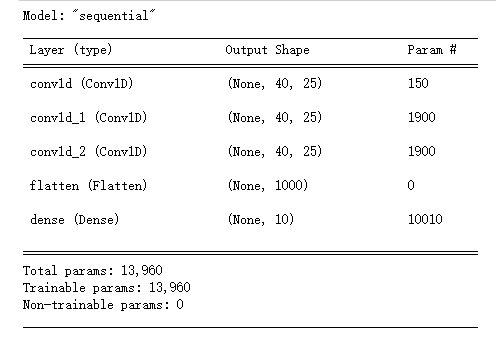
\includegraphics[width=0.5\textwidth]{T1Q1.png}
		\caption{Task1-Question1: ConvNet Model}
		\label{Fig.t1q1}
	\end{figure}
	
	This is not a complex network, since there are only three sequential convolution layer for feature extracting and no additional structures. The implementation code is as followed.
	
	\begin{lstlisting}
		weight_decay = 5e-4
		model = Sequential()
		#Your code starts from here 
		model.add(Input(shape=(40,1)))
		model.add(Conv1D(25, kernel_size=5, padding='same', activation='relu', kernel_regularizer=regularizers.l2(weight_decay)))
		model.add(Conv1D(25, kernel_size=3, padding='same', activation='relu', kernel_regularizer=regularizers.l2(weight_decay)))
		model.add(Conv1D(25, kernel_size=3, padding='same', activation='relu', kernel_regularizer=regularizers.l2(weight_decay)))
		
		model.add(Flatten())
		model.add(Dense(10, activation='softmax', kernel_initializer=keras.initializers.RandomNormal(mean=0.0, stddev=0.5),
		bias_initializer=keras.initializers.Zeros(), kernel_regularizer=regularizers.l2(weight_decay)))
		
		model.summary()
	\end{lstlisting}
	
	\subsection{Question 2}
	
	In this section, we applied the model constructed in the previous section to the MNIST1D dataset.\par
	
	In this part, we use the TensorBoard to record the training procedure, which we also found could be standalone execute as a TensorFlow based analyzing tool which is running on localhost with port 6006 by default.\par 
	% Can have a screenshot of the GUI here
	As a standard procedure using TensorFlow, first of all, we compile this model and set the loss function to cross-entropy, the optimizer to Stochastic Gradient Descent(SGD) and the target metrics to accuracy as required. \par
	Then we define a LearningRateScheduler, in order to control the learning rate during the training process. Learning rate is similar to a "step" of training process, which is typically set to 0.01 or 0.001. Learning rate only care about the magnitude, it somehow determine the precision of fitting parameters. In this part, we declare a dynamic learning rate to increase it speed to fit, while setting the magnitude to 0,01 according to the direction.\par
	For the next step, we declare the object of TensorBoard, along with the EarlyStopping to accomplish a speed-up of training working with the dynamic learning rate.
	\begin{figure}[h] 
		\centering
		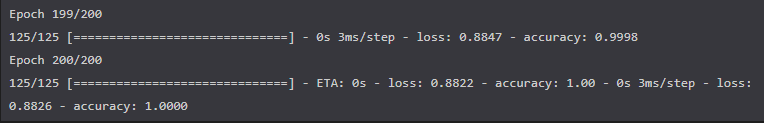
\includegraphics[width=0.5\textwidth]{T1Q2.png}
		\caption{Task1-Question2: Training Process Log} 
		\label{Fig.t1q2} 
	\end{figure}
	Then, in order to be convenient for the following steps, we extract the dataset into several lists, and handle the data into correct form. Finally, we feed the data with the facilities into the model to execute training process and save the model as a static file afterwards.\par
	A screen shot of the training log generated by TensorFlow is shown in Fig. 2.
	
	\begin{lstlisting}
		model.compile(loss=keras.losses.categorical_crossentropy,
		optimizer=tensorflow.keras.optimizers.SGD(),
		metrics=['accuracy'])
		
		def lr_scheduler(epoch):
		base_ep = 15
		return 1e-3 * (.5 ** (epoch // base_ep))
		lr_reduce_cb = keras.callbacks.LearningRateScheduler(lr_scheduler)
		tensorboard_cb = keras.callbacks.TensorBoard(log_dir='log2', write_graph=True)
		early_stopping_cb = keras.callbacks.EarlyStopping(patience=8, min_delta=0.)
		
		# X = tensorflow.expand_dims(dataset['x'],axis=2)
		train_x=dataset['x']
		train_y=dataset['y']
		train_x=train_x.reshape(4000,40,1)
		train_y=tensorflow.keras.utils.to_categorical(train_y, num_classes=10)
		
		# print(X.shape)
		history=model.fit(x=train_x,y=train_y,epochs=200,
		#                     steps_per_epoch=len(X) // 32,
		callbacks=[tensorboard_cb],                  
		shuffle = True,
		verbose=1)
		model.save('MNIST1D.h5')
	\end{lstlisting}
	
	
	
	
	\subsection{Question 3}
	
	In this section, we finish the typical model evaluation by extracting several significant statistics. As well-known and commonly used metrics, those statistics all have easy-to-run function to achieve, and most of them are from $scikit-learn$.
	
	\subsubsection{SubQuestion a}
	
	We firstly plot the loss curve and accuracy curve of the training process. As implementation, we extract the data using the training history, which is a return value of $model.fit()$. This is a modification of the original notebook since the $model.fit\_generator()$ is deprecated in TensorFlow 2.7.0 which is the version we used for this project, and it no longer saves training statistics of accuracy and loss during the training process in the log, which could be extracted by $tf\_record.tf\_record_iterator()$ in the past.\par
	As a matter of fact, this plot is generated only when we execute the training process (i.e. $model.fit()$ function). And it is shown in Fig. 3.
	
	\begin{figure}[h]
		\centering  %图片全局居中
		\subfigure[Loss]{
			\label{Fig.1loss}
			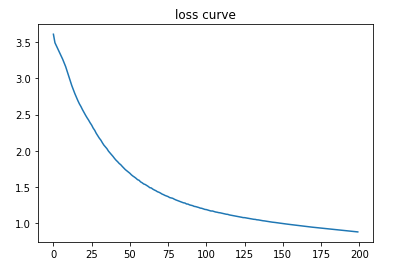
\includegraphics[width=0.4\textwidth]{T1Q3-b.png}}
		\subfigure[Accuracy]{
			\label{Fig.1acc}
			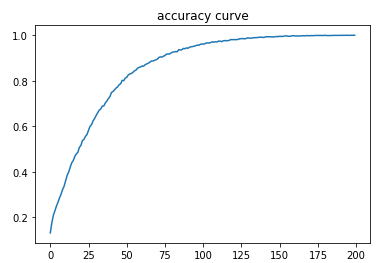
\includegraphics[width=0.4\textwidth]{T1Q3-a.png}}
		
		\caption{Loss and Accuracy Curve Plots on MNIST-1D dataset}
		\label{Fig.la}
	\end{figure}
	
	The code is quite simple as shown below, whose history object is define in the previous section as mentioned. 
	
	\begin{lstlisting}
		train_acc = history.history['accuracy']
		train_loss = history.history['loss']
		plt.plot(train_acc)
		plt.figure()
		plt.plot(train_loss)
	\end{lstlisting}
	
	\subsubsection{SubQuestion b}
	In this subquestion, our goal is to test the overall classification accuracy on the test set. As implementation, we first import test sets to $x\_test$ and $y\_test$ respectively. Then, we reshape the data in the $x\_test$. Next, we exploit $model.predict()$ to obtain the predicted output $y\_pred$. Finally, we compare the predicted values with the data in $y\_test$ to calculate the overall classification accuracy.\par
	\begin{figure}[h] 
		\centering
		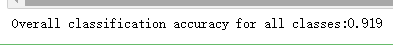
\includegraphics[width=0.5\textwidth]{T1Q3b.png}
		\caption{Task1-Question3b: Overall accuracy} 
		\label{Fig.t1q3b} 
	\end{figure}
	
	As a result, the overall accuracy is 0.919, which conforms to our expectation. Figure 4 shows the result of our experiment.\par
	
	
	
	The code used in this subquestion is showed below.
	
	\begin{lstlisting}
		# Use Scikit-learn to calculate stats
		from sklearn.metrics import accuracy_score, precision_score, recall_score,f1_score
		from sklearn.metrics import classification_report
		
		# Q3.b get the prediction from the test set
		x_test = dataset['x_test']
		y_test = dataset['y_test']
		x_test=x_test.reshape(1000,40,1)
		# predict_classes removed in tf 2.6.0
		y_pred = model.predict(x_test)
		y_predicted = np.argmax(y_pred,axis=1)
		print('Overall classification accuracy for all classes:'+str(np.sum(y_predicted==y_test)/y_test.shape[0]))
	\end{lstlisting}
	
	
	
	\subsubsection{SubQuestion c}
	In this subquestion, our goal is to test the classification accuracy of each class. For class $0$ to class $9$, we compute the accuracy respectively. Our code of this subquestion is showed below. We make use of the results of $y\_predicted$ in subquestion $b$. For each class, if $y\_predicted$ == $y\_test$, then we increment $res$, which is counter to record the number of samples that are classified correctly. Later, we can simply compute the accuracy by dividing $res$ by $true\_i.shape[0]$, which is the total sample number of class $i$.\par
	The code used in this subquestion is showed below.
	\begin{lstlisting}
		# Q3.c class-wise classification
		for i in range(10):
		true_i=np.where(y_test==i)[0]
		res=0
		for j in true_i:
		if y_predicted[j]==i:
		res=res+1
		print('class '+str(i)+' accuracy:'+str(res/true_i.shape[0]))
	\end{lstlisting} \par 
	We find the lines which belongs to class $i$ and find the ones which is correct in these lines to calculate the accuracy. The results of subquestion $b$ is showed in figure $5$.\par
	\begin{figure}[h] 
		\centering
		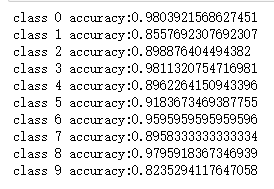
\includegraphics[width=0.35\textwidth]{T1Q3c.png}
		\caption{Task1-Question3b: class-wise accuracy} 
		\label{Fig.t1q3c} 
	\end{figure}
	
	
	As a result, class 0, class 3, class 5, class 6, class 8 have relatively higher accuracy, which are all greater than $90\%$, while class 1, class 2, class 4, class 7 and class 9 have relatively lower accuracy, which are all less than $90\%$.
	
	\begin{figure}[t]
		\centering  %图片全局居中
		\subfigure[Class 0]{
			\label{Fig.ROC0}
			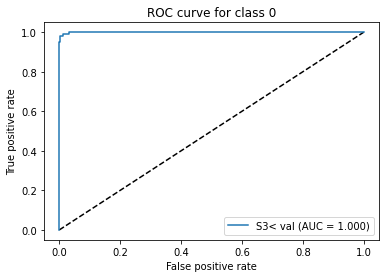
\includegraphics[width=0.23\textwidth]{ROC0.png}}
		\subfigure[Class 1]{
			\label{Fig.ROC1}
			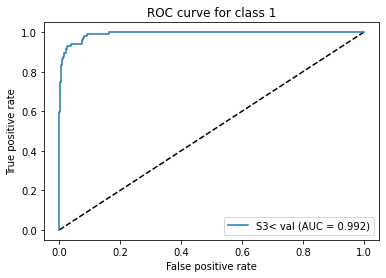
\includegraphics[width=0.23\textwidth]{ROC1.png}}
		\subfigure[Class 2]{
			\label{Fig.ROC2}
			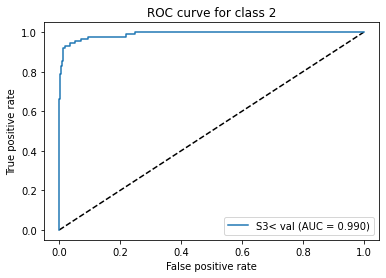
\includegraphics[width=0.23\textwidth]{ROC2.png}}
		\subfigure[Class 3]{
			\label{Fig.ROC3}
			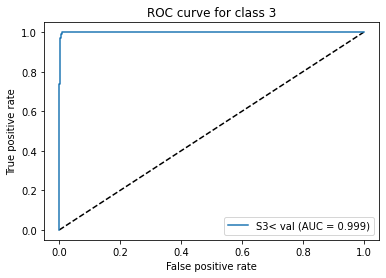
\includegraphics[width=0.23\textwidth]{ROC3.png}}
		\subfigure[Class 4]{
			\label{Fig.ROC4}
			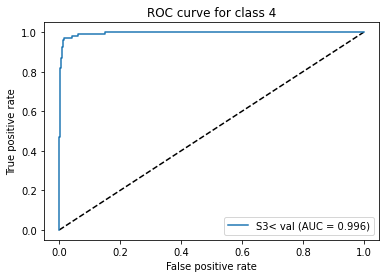
\includegraphics[width=0.23\textwidth]{ROC4.png}}
		\subfigure[Class 5]{
			\label{Fig.ROC5}
			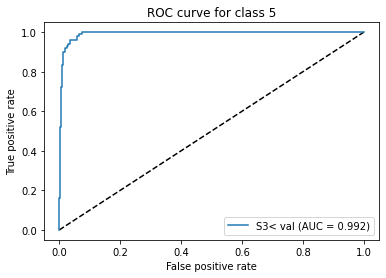
\includegraphics[width=0.23\textwidth]{ROC5.png}}
		\subfigure[Class 6]{
			\label{Fig.ROC6}
			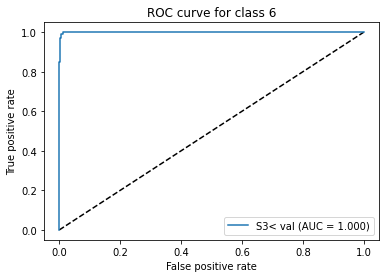
\includegraphics[width=0.23\textwidth]{ROC6.png}}
		\subfigure[Class 7]{
			\label{Fig.ROC7}
			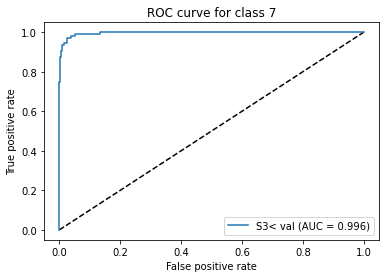
\includegraphics[width=0.23\textwidth]{ROC7.png}}
		\subfigure[Class 8]{
			\label{Fig.ROC8}
			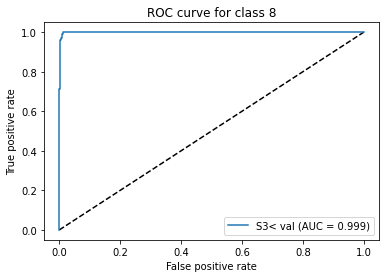
\includegraphics[width=0.23\textwidth]{ROC8.png}}
		\subfigure[Class 9]{
			\label{Fig.ROC9}
			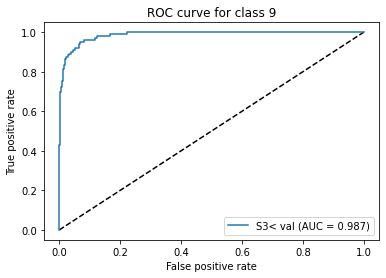
\includegraphics[width=0.23\textwidth]{ROC9.png}}
		
		\caption{Class-wise ROC Curve Plots on MNIST-1D dataset}
		\label{Fig.ba}
	\end{figure}
	\subsubsection{SubQuestion d}
	In this subquestion, our goal is to plot the $ROC$ and $AUC$ curves for each class. First of all, we transform the test set and reshape it to a 2D set. For each class, we compute the parameters $FPR$, $TPR$ by calling the function $roc\_curve$. Then we input the $FPR$ and $TPR$ parameters into function $auc()$, and obtained the returned value $AUC$, which is used to plot the graph.\par
	The code used in this subquestion is showed below.
	\begin{lstlisting}
		# Q3.d ROC and AUC curve for every class
		from sklearn.metrics import roc_curve
		from sklearn.metrics import auc
		# print(dataset['y_test'].shape)
		real_y=np.zeros((dataset['y_test'].size,10))
		for i in range(y_test.size):
		real_y[i,y_test[i]]=1
		for i in range(10):
		FPR, TPR, thresholds_keras = roc_curve(real_y[:,i], y_pred[:,i])   
		AUC = auc(FPR, TPR)
		print("AUC : ", AUC)
		plt.figure()
		plt.plot([0, 1], [0, 1], 'k--')
		plt.plot(FPR, TPR, label='S3< val (AUC = {:.3f})'.format(AUC))
		plt.xlabel('False positive rate')
		plt.ylabel('True positive rate')
		plt.title('ROC curve for class '+str(i))
		plt.legend(loc='best')
		plt.show()   
	\end{lstlisting}
	
	The AUC and ROC curves we plotted by executing the code are listed in figure $6$.
	
	
	\subsubsection{SubQuestion e}
	In this sebquestion, our goal is to plot the normalized confusion matrix.
    First, we will get the confusion matrix $cm$ using $confusion\_matrix$ function.
    We use $y_test$ which represents the real class labels of test set and $y_predicted$ which represents the predicted labels using the model.
    We transformed them as $list$ to fit into the function.
    Then we use $cm.astype('float') / cm.sum(axis=1)[:, np.newaxis]$ to normalize the confusion matrix.
    After that, we will set the plot cmap to blue confusion matrix plot, amd set the parameter in the plot $ax$.
    Finally, we will fit all the data in normalized confusion matrix into the data.
	The code used in this subquestion is showed below, and the result plot is displayed in figure 7.
	\begin{lstlisting}
		from sklearn.metrics import confusion_matrix
		cm=confusion_matrix(list(y_test),list(y_predicted))
		cm_normalized = cm.astype('float') / cm.sum(axis=1)[:, np.newaxis]
		fig, ax = plt.subplots()
		im = ax.imshow(cm, interpolation='nearest', cmap=plt.cm.Blues)
		ax.figure.colorbar(im, ax=ax)
		classes=[0,1,2,3,4,5,6,7,8,9]
		# print(classes)
		# We want to show all ticks...
		ax.set(xticks=np.arange(cm_normalized.shape[1]),
		yticks=np.arange(cm_normalized.shape[0]),
		# ... and label them with the respective list entries
		xticklabels=classes, yticklabels=classes,
		ylabel='True label',
		xlabel='Predicted label')
		plt.setp(ax.get_xticklabels(),  ha="right",
		rotation_mode="anchor")
		thresh = cm_normalized.max() / 2.
		for i in range(cm_normalized.shape[0]):
		for j in range(cm_normalized.shape[1]):
		ax.text(j, i, format(cm_normalized[i, j], '.2f'),
		ha="center", va="center",
		color="white" if cm_normalized[i, j] > thresh else "black")
		fig.tight_layout()
	\end{lstlisting}
	
	\begin{figure}[h] 
		\centering
		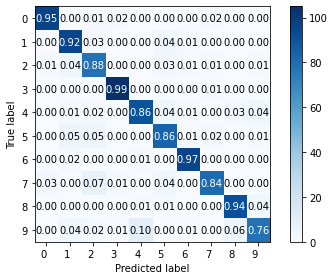
\includegraphics[width=0.3\textwidth]{T1Q3e.png}
		\caption{normalized confusion matrix plot}
		\label{Fig.t1q3e}
	\end{figure}
	\subsubsection{SubQuestion f}
	In this subquestion, our goal is to calculate Precision, Recall, and F-1 score on the test set. We call $classification\_report()$ to compute the statistics. \par
	
	The code used in this subquestion is showed below. \par
	
	
	
	\begin{lstlisting}
		# Q3.f
		print(classification_report(y_true=y_test,y_pred=y_predicted))
	\end{lstlisting} \par
	The result of the calculation is displayed in figure 8. As a result, the accuracy on total test set if 0.92, the f1-score is 0.92 and the recall is 0.92.
	\begin{figure}[h] 
		\centering
		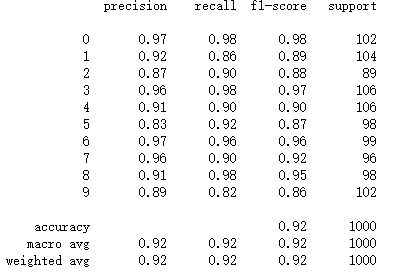
\includegraphics[width=0.4\textwidth]{T1Q3f.png}
		\caption{Precision,Recall and F-1 score}
		\label{Fig.t1q3f}
	\end{figure}
	\subsection{Question 4}
	To do this question, we did some coding in our program, the codes are listed below:
	
	Success Examples:
	\begin{lstlisting}
		index 10 true class: 0 predicted class: 0
		index 412 true class: 1 predicted class: 1
		index 729 true class: 2 predicted class: 2
	\end{lstlisting}
	Failure Examples:
	\begin{lstlisting}
		index 236 true class: 0 predicted class: 7
		index 6 true class: 1 predicted class: 2
		index 25 true class: 1 predicted class: 4
	\end{lstlisting}
	
	All the concrete Success/Failure cases are listed in 'MNIST1D.ipynb', if you want to refer to more examples.
	The most misclassification lies in class 1 and 9. It is obvious class-wise accuracy.
    There are several reasons for this. We think the most important reason is the unbalanced dataset. 
    We can see from $ROC$ curve. It is obvious that class 1 and class 9 has a worse ROC curve than other classes.
    The more AUC is closer to 1.0, the easier it will be to maintain a high precision and recall at the same time.
    And see from our results, we can clearly see from the ROC curve, the class 1 and 9 have the lowest AUC values.
    This is also shown in the $Question 3-f$, from the precision and recall table, we can see that the recall and precision is relatively lower than that of other classes.
    With low recall rate, the model cannot detect this class very well, and with a low precision, it's hard to trust its correctness when predicting this class.
    Class 9 has a lowest performance considering both precision and recall, so it has the lowest accuracy.To solve this, we can use undersampling, oversampling or generate synthetic data.\par
    The second reason is the overfitting on the training set. It's likely that if the design is too complex compared to the relatively simple dataset, it'll lead to overfitting. The training accuracy may be very high. However, the testing set will not get a high precision due to overfitting.


\section{Task 2: CNN interprectation}

This section introduces our interpretation of 1-D CNN model based on MNIST-1D dataset using 3 different attribution methods, including our literature review, discussion and implementation of the XAI attribute algorithms.

\subsection{Grad-CAM}
In the previous study, researchers introduced CAM to explain the CNN. However, CAM requires to modify the structure of original training models. It limits the usage of CAM greatly, because the cost of retraining the model is quite high for the published model. It is almost impossible to retrain them.
To solve this problem, Grad-CAM was proposed, which is similar to CAM. It also gets the weight of every feature maps and calculate the results accordingly. The difference lies in the calculation of weights. CAM replaced full-connection layer with GAP layer and retrain this whole model. In contrast to that, Grad-CAM put forward a new way to do it.
It calculates the weight by averaging the gradients which is equivalent to the CAM. It makes CAM applicable to all the existing models.\par

The core algorithm of Grad-CAM is based on CAM which proposed: class c gets the final classification score $Y_{c}$ with a linear combination of its global average pooled last convolutional layer feature maps $A_{k}$.

\begin{equation}
    \begin{aligned}
        Y^{c}=\Sigma_{k}w_{k}^{c}\Sigma_{i}\Sigma_{j}A_{ij}^{k}
        \label{Grad-CAM_Y}
    \end{aligned}
  \end{equation}

So, first, it defines the weight of feature map $k$ to class $c$ as $\alpha_{k}^{c}$, and it calculates the weight using the global gradients\ref{Grad-CAM_alpha}:
\begin{equation}
    \begin{aligned}
        \alpha_{k}^{c}=\frac{1}{Z}*\Sigma_{i}\Sigma_{j}\frac{\partial y^{c}}{\partial A_{ij}^{k}}
        \label{Grad-CAM_alpha}
    \end{aligned}
  \end{equation}
  In which, $y_{c}$ is the gradient of the score for class c, $A_{k}$ is the feature map activation.$\frac{\partial y^{c}}{\partial A_{ij}^{k}}$ is the gradient achieved by backpropagating. $\frac{1}{Z}$ is global averaging.
  After calculating the $\alpha_{k}^{c}$, the algorithm computed the weighted combination of forward activation maps, followed by a ReLU function:

$$L_{Grad-CAM}^{c}=ReLU(\Sigma_{k}\alpha_{k}^{c}A^{k})$$

The advantages for Grad-CAM is quite obvious: First, compared with CAM, it does not need to change the model and retrain it which costs a lot of time and money. 
The novelty is the usage of propagation and gradients to compute the weights of feature maps.It makes the visualization of published models possible. Second is that the algorithm is quite easy to code and maintain.\par
The disadvantages for Grad-CAM is that: it considers the global features for all classes. As a result, Grad-CAM cannot localize the targets when faced with many targets of the same class. If there are many objects of the same class in an image, it cannot localize the targets well or it can only locate part of them.

\subsection{Grad-CAM++}
Grad-CAM++ is an algorithm based on Grad-CAM, aiming to get a better explanation for CNN models. It improves the performance of Grad-CAM when facing targets of the same class, and helps to better localize the targets.\par
It introduced a weighted combination of gradients of the output in the pixel level, which provides a measure of importance of every pixels to the feature maps.
It introduced a closed-form solution for the pixels weights, thus making the improvement of explanation possible. \par
The core algorithm is shown below:
First, as we have introduced above, class c gets the final classification score $Y_{c}$ with a linear combination of its global average pooled last convolutional layer feature maps $A_{}k$ in equation\ref{Grad-CAM_alpha}.
Grad-CAM calculates the weight $w_{k}^{c}$ with equation\ref{Grad-CAM_weight}.  To improve the performance, Grad-CAM++ changed this equation.
Combine the equation\ref{Grad-CAM_alpha} and \ref{Grad-CAM-1} together, we will get the equation\ref{Grad-CAMPP-1}:
\begin{equation}
    \begin{aligned}
        Y^{c}=\Sigma_{k}[\Sigma_{i}\Sigma_{j}(\Sigma_{a}\Sigma_{b}\alpha_{ab}^{kc}·relu(\frac{\partial Y_{c}}{\partial A_{ab}^{k}}))A_{ij}^{k}]
        \label{Grad-CAMPP-1}
    \end{aligned}
\end{equation}
Take partial derivative w.r.t. $A_{ij}^{k}$ on both sides:
\begin{equation}
\begin{aligned}
\frac{\partial Y_{c}}{\partial A_{ij}^{k}}=\Sigma_{a}\Sigma{b}\alpha_{ab}^{kc}·\frac{\partial Y_{c}}{\partial A_{ab}^{k}}+\Sigma_{a}\Sigma{b}A_{ab}^{k}\{\alpha_{ij}^{kc}·\frac{\partial^{2} Y_{c}}{(\partial A_{ij}^{k} )^{2}}\}
\label{Grad-CAMPP-2}
\end{aligned}
\end{equation}
Take a further partial derivative w.r.t. $A_{ij}^{k}$ on both sides:
\begin{equation}
    \begin{aligned}
\frac{\partial^{2} Y_{c}}{(\partial A_{ij}^{k})^{2}}=2·\alpha_{ij}^{kc}·\frac{\partial^{2} Y_{c}}{(\partial A_{ij}^{k})^{2}}+\Sigma_{a}\Sigma{b}A_{ab}^{k}\{\alpha_{ij}^{kc}·\frac{\partial^{3} Y_{c}}{(\partial A_{ij}^{k})^{3}}\}
        \label{Grad-CAMPP-3}
    \end{aligned}
    \end{equation}
Rearrage equation\ref{Grad-CAMPP-3}, we get:
    \begin{equation}
        \begin{aligned}
\alpha_{ij}^{kc}=\frac{\frac{\partial^{2} Y_{c}}{(\partial A_{ij}^{k})^{2}}}{2\frac{\partial^{2} Y_{c}}{(\partial A_{ij}^{k})^{2}}+\Sigma_{a}\Sigma{b}A_{ab}^{k}\{\frac{\partial^{3} Y_{c}}{(\partial A_{ij}^{k})^{3}}\}}
            \label{Grad-CAMPP-4}
        \end{aligned}
        \end{equation}
So, we are able to get weight $w_{k}$ with:
\begin{equation}
    \begin{aligned}
        w_{k}^{c}=\Sigma_{i}\Sigma_{j}\alpha_{ij}^{kc}·relu(\frac{\partial Y_{c}}{\partial A_{ij}^{k}})
        \label{Grad-CAMPP-5}
    \end{aligned}
    \end{equation}

Applying equation\ref{Grad-CAMPP-5} to \ref{Grad-CAM_weight}, we will get final results.
There are many advantages for Grad-CAM++: First, it clearly improved the performance of Grad-CAM when facing with many objects of the same class in an image. It helps us to localize the objects more accurately. 
Second is that it only adds tow partial derivative to the computation, and it uses backpropagation only once. So it does not increase the computation time a lot.\par
However, it still remains to be revised in some aspects: First, although it improved the performance of Grad-CAM in some degrees, its performance is far from perfect. The same problem remains and connot be solved completelly. 
Second, from my perspective, ignoring the relu function in the alpha calculation will decrease the precision.\par
Our implementation code is as followed:
\begin{lstlisting}
    ef grad_cam_plus_plus(input_model, image, layer_name, class_index=None):
    # if class_index is None:
    #     class_index=np.argmax(input_model.predict(np.array([image])), axis=-1)[0]
    """GradCAM method for visualizing input saliency."""
    # cls = np.argmax(input_model.predict(image))
    y_c = input_model.output
    conv_output = input_model.get_layer(layer_name).output
    feedforward1 = keras.models.Model([input_model.input], [conv_output, y_c])
    # with tf.GradientTape() as tape1:
    #     with tf.GradientTape() as tape2:
    #         with tf.GradientTape() as tape3:
    #             ff_results = feedforward1([image])
    #             all_fmap_masks, predictions = ff_results[0], ff_results[-1]
    if class_index==None:
        cls=np.argmax(input_model.predict(image))
    else:
        cls=class_index
    #             loss = predictions[:, cls]
    #         grads_val = tape3.gradient(loss, all_fmap_masks)
    #     grads_val2 = tape2.gradient(grads_val, all_fmap_masks)
    # grads_val3 = tape1.gradient(grads_val2, all_fmap_masks)
    with tf.GradientTape() as tape:
        ff_results=feedforward1([image])
        all_fmap_masks, predictions = ff_results[0], ff_results[-1]
        loss = predictions[:, cls]
    grads_val = tape.gradient(loss, all_fmap_masks)
    grads_val2=grads_val**2
    grads_val3=grads_val2*grads_val
    if len(image.shape) == 3:
        axis = (0, 1)
    elif len(image.shape) == 4:
        axis = (0, 1, 2)
    alpha_div=(2.0 * grads_val2 + grads_val3 * np.sum(all_fmap_masks, axis))
    alpha_div = np.where(alpha_div != 0.0, alpha_div, 0)
    alpha = grads_val2 / alpha_div
    weights = np.maximum(grads_val, 0.0) * alpha
    weights = np.sum(weights, axis=axis)
    # weights = np.mean(grads_val, axis=axis)
    cam = np.dot(all_fmap_masks[0], weights)
    # print (cam)
    H, W = image.shape[1:3]
    cam = np.maximum(cam, 0)
    # cam = resize(cam, (H, W))
    cam = zoom(cam, H / cam.shape[0])
    # cam = np.maximum(cam, 0)
    cam = cam / cam.max()
    return cam
\end{lstlisting}
\subsection{Ablation-CAM}

The Ablation-CAM creatively uses ablation analysis to determine the importance of individual feature map units for different classes. It proposes a novel “gradient-free” visualization approach which avoids use of gradients and at the same time, produce high quality class-discriminative localization maps.\par

The core algorithm of Ablation-CAM is not complex: it uses the value of slope to describe the effect of ablation of individual unit $k$ by the following formula:

$$slope = \frac{y^c-y^c_k}{||A_k||}$$

In the formula, $y^c$ stands for activation score of class c, which represent the entire class activation status. $y^c_k$ indicates the value of the function for absence of unit $k$, where $A_k$ is the baseline. Those concepts lead us to ablation study, which is the basic principle of the method.\par
Ablation study is a method to distribute the influencing importance of different factors by controlling the variable while switching the combination of potential factors, and also their standalone. For example, if we'd like to know whether $A$ or $B$ component of medicine could improve the effect of an old medicine $C$. We could compare $C+A$, $C+B$ and also $C+A+B$ with the baseline of $C$. We could know if the A or B or they together are able to improve the effect. In the instance of Ablation-CAM, different unit $k$ is the "component", and the whole feature map is so-called baseline, $A_k$. Thus, using slope described in the previous formula could represent the importance of a single unit to the feature map.\par
However practically, norm $||A_k||$ is hard to compute due to its large size and hence the slope could be approximately presented by the following formula, assuming a very small value.

$$w^c_k = \frac{y^c-y^c_k}{y^c}$$

As the algorithm, Ablation-CAM can then be obtained as weighted linear combination of activation maps and corresponding weights from the formula above, which is somehow similar to that of Grad-CAM.

$$L^C_{Ablation-CAM}=ReLU(\sum_k {w^c_k}{A_k})$$

There are a number of advantages and features of Ablation-CAM. Firstly, a significant contribution and novelty of the Ablation-CAM is the ablation analysis it used to decide the weights of feature map units. Secondly, it could produce a coarse localization map highlighting the regions in the image for prediction. Thirdly, compare to other CAM methods, this approach works essentially better when it is full connected to obtain the result, which is known as final linear classifier, and have as good performance as other gradient-based CAM methods when evaluating other CNNs. Last but not the least, the approach introduce a gradient-free principle which avoids use of gradient as Grad-CAM does and produce a high-quality class-wise localization maps, which helps it to adapt into any CNN based architecture.\par
However, the approach have some limitations as well. First of all, the computational time required to generate a single Ablation-CAM is much grater than the required for Grad-CAM, as it has to iterate over each feature map to ablate it and check the drop in class activation score correspondingly. 
On the hand, the Ablation-CAM only benefits the interpretation where last convolutional layer is not followed immediately by decision nodes, yet show the same performance statistically as other CAM methods.\par

Our implementation code is as followed.

\begin{lstlisting}
def extract_feature_map(img, model, class_index=None, layer_name="conv1d_2"):
    # Get gradients for the class on the last conv layer
    gradModel = tf.keras.models.Model([model.inputs],[model.get_layer(layer_name).output, model.output])
    print("gradModel = ")
    print(gradModel)
    # Get Activation Map on the last conv layer
    with tf.GradientTape() as tape:
        # Get Prediction on the last conv layer
        convOutputs, predictions = gradModel(np.array([img]))
        output = convOutputs[0]
        print("#prediction#")
        print(predictions)
        print("OUTPUT")
        print(output)
    
    if class_index is None:
        class_index = np.argmax(model.predict(np.array([img])), axis = -1)[0]
        y_class = np.max(model.predict(np.array([img])))
    else:
        y_class = model.predict(np.array([img]))[0][class_index]

    # Get Weights on the layer
    weights = np.zeros(model.get_layer(layer_name).get_weights()[1].shape)
    # Get Weights for the maps
    allWeights = model.get_layer(layer_name).get_weights().copy()
    zeroWeight = allWeights[0][:,:,:,0]*0
    localWeight = [np.zeros(allWeights[0].shape)]
    localWeight.append(np.zeros(allWeights[1].shape))

    for i in range(weights.shape[0]):
        localWeight[0] = allWeights[0].copy()
        localWeight[0][:,:,:,i] = zeroWeight
        model.get_layer(layer_name).set_weights(localWeight)
        y_pred = model.predict(np.array([img]))[0][class_index]
        weights[i] = (y_class - y_pred)/y_class # Simplified Formula
        model.get_layer(layer_name).set_weights(allWeights)

    outputMean = np.mean([output[:,:,i] for i in range(output.shape[2])], axis = 0)
    outputMean = np.maximum(outputMean, 0.0)
    outMeanMask = np.zeros(output.shape[0:2], dtype = np.float32)
    for i in range(output.shape[0]):
        for j in range(output.shape[1]):
            if outputMean[i][j] < np.mean(outputMean[:,:]):
                outMeanMask[i][j] = 255
            else:
                outMeanMask[i][j] = 0
    return weights, output, outputMean, outMeanMask

def ablation_cam(weights, output):
    ablationMap = weights * output
    ablationCam = np.sum(ablationMap, axis=(2))

    ablationMask = np.zeros(ablationMap.shape[0:2], dtype = np.float32)
    for i in range(ablationMap.shape[0]):
        for j in range(ablationMap.shape[1]):
            if ablationCam[i][j] < np.mean(ablationCam[:,:]):
                ablationMask[i][j] = 255
            else:
                ablationMask[i][j] = 0
    
    return ablationCam, ablationMask
\end{lstlisting}

\section{Task 3: Biomedical image classification and interpretation}
In this task, we basically apply the previous evaluation codes on HMT dataset with a 2-D CNN model following typical procedure, including plotting of test and attribution methods selected.
\subsection{Question 1}
In this section, we finish the typical model evaluation as we did in task 1 by extracting several significant statistics.As well-known and commonly used metrics, those statistics all have easy-to-run
function to achieve, and most of them are from $scikit-learn$.
\subsubsection{Overall classification accuracy}
First of all, we implemented the overall classification accuracy evaluation. We load the model trained before, use the $test\_generator.classes$ function to get the test set for labels which is noted as $y\_test$.
Then, we use the test_generator to predict the results with this model, the result names $y\_pred$. To achieve the label from the predict results, we then apply $np.argmax$ function to $y\_pred$ in every row and get the predicted label $y\_predicted$. 
So, for the overall classification accuracy, we need to compare the predicted labels with the true labels, calculate the number of pairs which have the same label.The function is realized by $np.sum(y\_predicted==y_test)$, and divide it with $y\_test.shape[0]$ which represents the amount of overall data, we will get the overall accuracy.
Here is the code:
\begin{lstlisting}
    from sklearn.metrics import accuracy_score, precision_score, recall_score,f1_score
    from sklearn.metrics import classification_report
    from sklearn.metrics import roc_curve, auc
    from sklearn.metrics import confusion_matrix

    test_generator.reset()
    y_test=test_generator.classes
    y_pred=model.predict(test_generator)
    y_predicted=np.argmax(y_pred, axis=1)
    print('Overall classification accuracy for all classes:'+str(np.sum(y_predicted==y_test)/y_test.shape[0]))
\end{lstlisting}
The result is 83.06\%,which conforms to our expectation. The result is shown in Fig\ref{Fig.t3q1}:
\begin{figure}[h] 
    \centering
    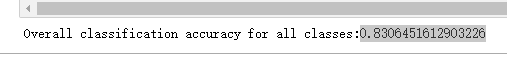
\includegraphics[width=0.4\textwidth]{T3Q1a.png}
    \caption{Overall classification accuracy}
    \label{Fig.t3q1}
\end{figure}
\subsubsection{class-wise classification accuracy}
In this part, we aim to discuss the classification accuracy for every class using the test set. 
For class $0$ to $7$, we use similar methods as the work in overall classification accuracy. 
We uses the results of $y\_test$ in the previous code which represents the real class of the test set. For every class, we firstly select from the test set which has the same label as current index $i$.
We uses $np.where$ function to get this. Then we will calculate the number of predicted labels in the index which hit the right labels. We use $res$ as a counter to do that.
For each class, if $y\_predicted == y\_test$, then we increment $res$.
Later, we can simply compute the accuracy by dividing $res$ by $true\_i.shape[0]$,which is the total sample number of class $i$.
Here is the code:
\begin{lstlisting}
    for i in range(8):
    true_i=np.where(y_test==i)[0]
    res=0
    for j in true_i:
        if y_predicted[j]==i:
            res=res+1
    print('class '+str(i)+' accuracy:'+str(res/true_i.shape[0]))
\end{lstlisting}
As a result, class 0, class 1, class 5, class 6, class 7 have relatively higher accuracy, which are all greater than $90\%$, while class 2, class 3, class 4 have relatively lower accuracy, which are all less than $90\%$.
The results are shown in Fig\ref{Fig.t3q2}:
\begin{figure}[h] 
    \centering
    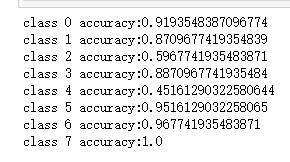
\includegraphics[width=0.3\textwidth]{T3Q1b.png}
    \caption{class-wise classification accuracy} 
    \label{Fig.t3q2} 
\end{figure}
\subsubsection{AUC-ROC curve}
In this part,o ur goal is to plot the $AUC$ and $ROC$ curves for each class.
First of all, we transform the test set label to a 2D set, in which only the value in real label index is set to 1.
Then we compute the FPR and TPR for each class by calling $roc_curve$ function.
After that, we fit the FPR and TPR into the funtion auc(), and obtained the returned value $AUC$, which is used in the plot.\par
Here is the code:
\begin{lstlisting}
    real_y=np.zeros((y_test.size,8))
    for i in range(y_test.size):
        real_y[i,y_test[i]]=1
    for i in range(8):
        FPR, TPR, thresholds_keras = roc_curve(real_y[:,i], y_pred[:,i]) 
        AUC = auc(FPR, TPR)  
        print("AUC for class "+str(i)+": ", AUC)
        plt.figure()
        plt.plot([0, 1], [0, 1], 'k--')
        plt.plot(FPR, TPR, label='S3< val (AUC = {:.3f})'.format(AUC))
        plt.xlabel('False positive rate')
        plt.ylabel('True positive rate')
        plt.title('ROC curve for class '+str(i))
        plt.legend(loc='best')
        plt.show()    
\end{lstlisting}

The AUC and ROC curves we plotted by executing the code are listed in in Fig. 11.

\begin{figure}[h]
\centering  
\subfigure[Class 0]{
\label{Fig.3ROC0}
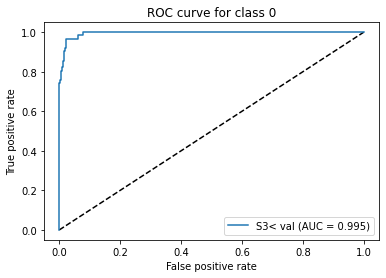
\includegraphics[width=0.2\textwidth]{3ROC0.png}}
\subfigure[Class 1]{
\label{Fig.3ROC1}
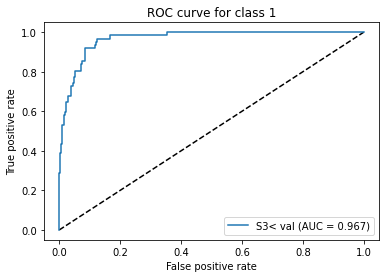
\includegraphics[width=0.2\textwidth]{3ROC1.png}}
\subfigure[Class 2]{
\label{Fig.3ROC2}
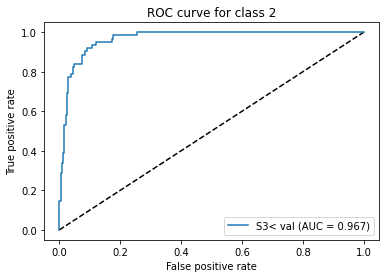
\includegraphics[width=0.2\textwidth]{3ROC2.png}}
\subfigure[Class 3]{
\label{Fig.3ROC3}
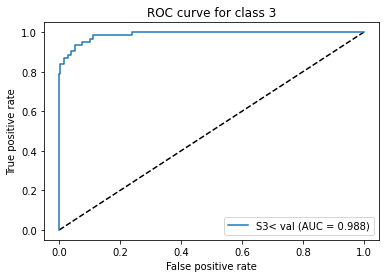
\includegraphics[width=0.2\textwidth]{3ROC3.png}}
\subfigure[Class 4]{
\label{Fig.3ROC4}
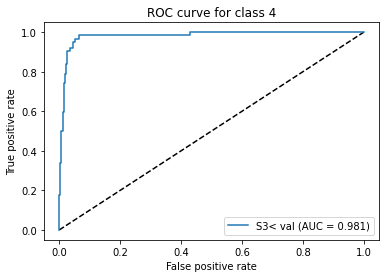
\includegraphics[width=0.2\textwidth]{3ROC4.png}}
\subfigure[Class 5]{
\label{Fig.3ROC5}
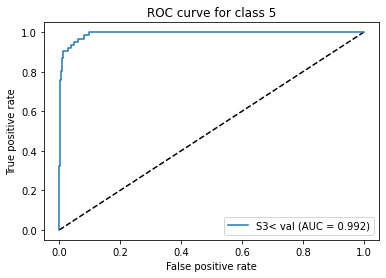
\includegraphics[width=0.2\textwidth]{3ROC5.png}}
\subfigure[Class 6]{
\label{Fig.3ROC6}
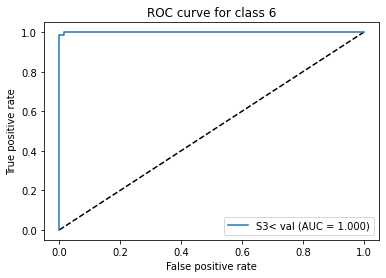
\includegraphics[width=0.2\textwidth]{3ROC6.png}}
\subfigure[Class 7]{
\label{Fig.3ROC7}
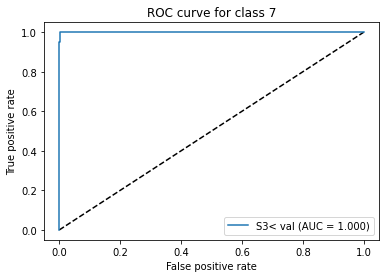
\includegraphics[width=0.2\textwidth]{3ROC7.png}}


\caption{Class-wise ROC Curve Plots of HMT dataset}
\label{Fig.ba}
\end{figure}

\subsubsection{normalized confusion matrix}
In this part, we aim to plot the normalized confusion matrix.
First, we will get the confusion matrix $cm$ using $confusion\_matrix$ function.
We use $y_test$ which represents the real class labels of test set and $y_predicted$ which represents the predicted labels using the model.
We transformed them as $list$ to fit into the function.
Then we use $cm.astype('float') / cm.sum(axis=1)[:, np.newaxis]$ to normalize the confusion matrix.
After that, we will set the plot cmap to blue confusion matrix plot, amd set the parameter in the plot $ax$.
Finally, we will fit all the data in normalized confusion matrix into the data.
Here is the code:
\begin{lstlisting}
    cm=confusion_matrix(list(y_test),list(y_predicted))
    cm_normalized = cm.astype('float') / cm.sum(axis=1)[:, np.newaxis]
    fig, ax = plt.subplots()
    im = ax.imshow(cm, interpolation='nearest', cmap=plt.cm.Blues)
    ax.figure.colorbar(im, ax=ax)
    classes=[0,1,2,3,4,5,6,7]
    # print(classes)
    # We want to show all ticks...
    ax.set(xticks=np.arange(cm_normalized.shape[1]),
        yticks=np.arange(cm_normalized.shape[0]),
        # ... and label them with the respective list entries
        xticklabels=classes, yticklabels=classes,
        ylabel='True label',
        xlabel='Predicted label')
    plt.setp(ax.get_xticklabels(),  ha="right",
                rotation_mode="anchor")
    thresh = cm_normalized.max() / 2.
    for i in range(cm_normalized.shape[0]):
        for j in range(cm_normalized.shape[1]):
            ax.text(j, i, format(cm_normalized[i, j], '.2f'),
                    ha="center", va="center",
                    color="white" if cm_normalized[i, j] > thresh else "black")
    fig.tight_layout()
\end{lstlisting}
The result plot is shown in Fig.\ref{Fig.t3q1c}.
\begin{figure}[h] 
    \centering
    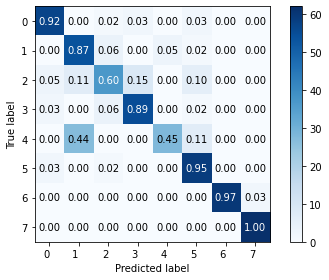
\includegraphics[width=0.4\textwidth]{T3Q1c.png}
    \caption{normalized confusion matrix plot} 
    \label{Fig.t3q1c} 
\end{figure}

\subsubsection{Precision, Recall, and F-1 score}
In this part, our goal is to calculate Precision, Recall, and F-1 score on the test set. We call
$classification\_report()$ to compute the statistics. Here is the code:
\begin{lstlisting}
    print(classification_report(y_true=y_test,y_pred=y_predicted))
\end{lstlisting}
The result plot is shown in Fig.\ref{Fig.t3q1d}.As a result, the accuracy on total test set if 0.85, the f1-score is 0.83 and the recall is 0.82
\begin{figure}[h] 
    \centering
    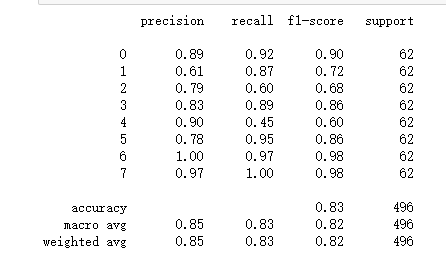
\includegraphics[width=0.5\textwidth]{T3Q1d.png}
    \caption{Precision, Recall, and F-1 score} 
    \label{Fig.t3q1d} 
\end{figure}

\subsection{Question 2}

%implement 2d capable functions.
In this section, we describe the implementation of attribution methods application in HMT. As mentioned before, HMT is a 2-Dimensional based dataset, and therefore we need to either develop a capable XAI methods taking both 3-Dimensional and 4-dimensional tensor corresponding to 1-D and 2-D dataset, or we set up separate methods dealing with 2-Dimensional dataset, HMT. In our implementation, we choose different option for the two methods.\par

Our Grad-CAM++ implementation is a capable function whose code is as followed.

\begin{lstlisting}
def grad_cam_plus_plus(input_model, image, layer_name, class_index=None):
    # if class_index is None:
    #     class_index=np.argmax(input_model.predict(np.array([image])), axis=-1)[0]
    """GradCAM method for visualizing input saliency."""
    cls = np.argmax(input_model.predict(image))
    y_c = input_model.output
    conv_output = input_model.get_layer(layer_name).output
    feedforward1 = keras.models.Model([input_model.input], [conv_output, y_c])
    # with tf.GradientTape() as tape1:
    #     with tf.GradientTape() as tape2:
    #         with tf.GradientTape() as tape3:
    #             ff_results = feedforward1([image])
    #             all_fmap_masks, predictions = ff_results[0], ff_results[-1]
    if class_index==None:
        cls=np.argmax(input_model.predict(image))
    else:
        cls=class_index
    #             loss = predictions[:, cls]
    #         grads_val = tape3.gradient(loss, all_fmap_masks)
    #     grads_val2 = tape2.gradient(grads_val, all_fmap_masks)
    # grads_val3 = tape1.gradient(grads_val2, all_fmap_masks)
    with tf.GradientTape() as tape:
        ff_results=feedforward1([image])
        all_fmap_masks, predictions = ff_results[0], ff_results[-1]
        loss = predictions[:, cls]
    grads_val = tape.gradient(loss, all_fmap_masks)
    grads_val2=grads_val**2
    grads_val3=grads_val2*grads_val
    if len(image.shape) == 3:
        axis = (0, 1)
    elif len(image.shape) == 4:
        axis = (0, 1, 2)
    alpha_div=(2.0 * grads_val2 + grads_val3 * np.sum(all_fmap_masks, axis))
    alpha_div = np.where(alpha_div != 0.0, alpha_div, 0)
    alpha = grads_val2 / alpha_div
    weights = np.maximum(grads_val, 0.0) * alpha
    weights = np.sum(weights, axis=axis)
    # weights = np.mean(grads_val, axis=axis)
    cam = np.dot(all_fmap_masks[0], weights)
    # print (cam)
    H, W = image.shape[1:3]
    cam = np.maximum(cam, 0)
    # cam = resize(cam, (H, W))
    cam = zoom(cam, H / cam.shape[0])
    # cam = np.maximum(cam, 0)
    cam = cam / cam.max()
    return cam
\end{lstlisting}

The capability is achieved by the code of branch,
\begin{lstlisting}
    if len(image.shape) == 3:
        axis = (0, 1)
    elif len(image.shape) == 4:
        axis = (0, 1, 2)
\end{lstlisting}
and hence it is able to process both 3-Dimensional and 4-Dimensional tensors.

Another modification needs to be mentioned is that there is a slightly modification practically in the implementation. It is modified due to troubleshooting of HMT explanation. The origin function gives an extremely unsatisfying result thus we change the way we calculate secondary gradient and third gradient. We use multiplication instead of slope to get the gradient value due to its low magnitude, the absolute value of both results are similar, however the multiplication is positive constantly.\par
There are some potential reasons we could come up with.
%codes

%modifications

\section{Task 4: Quantitative evaluation of the attribution methods}

In this task, we use two rates, decrease rate and increase rate, to evaluate the explanation map generated by the attribution methods, in order to assess the performance of the methods we implemented. Besides, we would like to use some subjective observation to evaluate the performance as a supportive evaluation.

\subsection {Experiment}

The calculator function is already provided in the notebook, which takes in a 3-Dimensional map for MNIST-1D dataset and deals with a 4-Dimensional explanation map for HMT dataset. However, we have the processing codes slightly modified, which is shown below.

An example of Grad-CAM++ rate calculation procedure in MNIST-1D dataset is as followed. Note that the explanation map should be reshape to $(40,1)$ in order to fix in the calculator, or otherwise the explanation map has a $(40,)$ shape. We run 100 times to get a sampling result of the rates.

\begin{lstlisting}
drop_rate = 0.
increase_rate = 0.
temp=np.expand_dims(x_test[0], axis=0)
print(np.expand_dims(x_test[0], axis=0).shape)
for index in range(100):
#     print(np.expand_dims(np.expand_dims(x_test[index], axis=0), axis=-1).shape)
    # print(index)
    prediction=model(np.expand_dims(x_test[index], axis=0)).numpy()
    explanation_map = grad_cam(model, np.expand_dims(x_test[index], axis=0),  layer_name='conv1d_2')
    # print(explanation_map.shape)
    explanation_map = np.reshape(explanation_map, (40,1))
    res = calculate_drop_increase(np.expand_dims(x_test[index], axis=0), model, explanation_map, class_index=np.argmax(prediction[0]), frac=0.3)
    drop_rate += res[0]
    increase_rate += res[1]
drop_rate /= 100
increase_rate /= 100
print(drop_rate)
print(increase_rate)
\end{lstlisting}

An example of Grad-CAM rate calculation procedure in HMT dataset is as followed. Similar to the procedure structure in MNIST-1D, we firstly initialize the variables and reset the generator. Then recursively, we generate explanation map for 15 batches, and 32 samples per batch, and calculate both the drop and increase rate by the calculator function. To get the averaged value, which is the rate, we firstly add them up to the variable and finally divided by the total running times. Specifically, we set the parameter $frac$ to 0.9 as required in HMT datasets.

\begin{lstlisting}
test_generator.reset()
drop_rate = 0.
increase_rate = 0.
for i in range(15):
    image_batch,label_batch=test_generator.next()
    # print("Current Round:", i)
    for index in range(32):
        # print(i, index)
        prediction=model(image_batch)
        explanation_map_GradCAM = grad_cam(model, np.expand_dims(image_batch[index], axis=0), 'max_pooling2d_1')
        res = calculate_drop_increase(np.expand_dims(image_batch[index], axis=0), model, explanation_map_GradCAM, class_index=np.argmax(prediction[index]), frac=0.9)

        drop_rate += res[0]
        increase_rate += res[1]

drop_rate /= (15*32)
increase_rate /= (15*32)
print("======Grad-CAM======")
print(drop_rate, increase_rate)
\end{lstlisting}

Specially, for the ablation-CAM, we could only implement it and generate explanation map in the last convolution layer which is different with other maps and have a different size (112,112) correspondingly. So alternatively, the calculation process of ablation-CAM is shown as followed, in which we add a resize function to force it fit in the layer size.

\begin{lstlisting}
drop_rate = 0.
increase_rate = 0.

for i in range(15):
    image_batch,label_batch=test_generator.next()
    print("Current Round:", i)
    for index in range(32):
        # print(i, index)
        prediction=model(image_batch)
        explanation_map_ablation_cam = ablation_cam_2d(model, np.expand_dims(image_batch[index], axis=0), 'conv2d_3')
        explanation_map_ablation_cam = cv2.resize(explanation_map_ablation_cam, (224,224), interpolation=cv.INTER_AREA)
        res = calculate_drop_increase(np.expand_dims(image_batch[index], axis=0), model, explanation_map_ablation_cam, class_index=np.argmax(prediction[index]), frac=0.9)

        drop_rate += res[0]
        increase_rate += res[1]

drop_rate /= (15*32)
increase_rate /= (15*32)
print("======Ablation-CAM======")
print(drop_rate, increase_rate)
\end{lstlisting}

We can get all the rates after rounds of experiment, and the data is shown in the table.

\begin{table}[h]
\caption{Drop and Increase Rates of Different attribution Methods in MNIST-1D and HMT}
\begin{tabular}{|l|l|l|}
\hline
Rate                    & Drop Rate (\%) & Increase Rate (\%) \\ \hline
Grad-CAM (MNIST-1D)     & 36.980         & 33.000             \\ \hline
Grad-CAM++ (MNIST-1D)   & 21.964         & 27.000             \\ \hline
Ablation-CAM (MNIST-1D) & 19.715         & 32.000             \\ \hline
Grad-CAM (HMT)          & 47.436         & 22.083             \\ \hline
Grad-CAM++ (HMT)        & 50.921         & 19.792             \\ \hline
Ablation-CAM (HMT)      & 43.341         & 30.469             \\ \hline
\end{tabular}
\end{table}

From the table we could know that in HMT, Ablation-CAM works best, as it has lowest drop rate among the algorithms and highest increase rate. Besides in MNIST-1D dataset, ablation-CAM also shows greater performance than the other CAM-based attribution methods, which probably means it will be a good choice in some specific scenarios.\par
We will further discuss the evaluation result in the next section.

\subsection{Discussion}

data analysis

successful? compare to benchmark

fail?

Two methods comparison.

\begin{thebibliography}{00}
\bibitem{b1}Y. Gilad, R. Hemo, S. Micali, G. Vlachos, and N. Zeldovich, “Algorand: Scaling Byzantine Agreements for Cryptocurrencies,” in Proceedings of the 26th Symposium on operating systems principles, 2017, pp. 51–68. doi: 10.1145/3132747.3132757.
\bibitem{b2} King, Sunny, and Scott Nadal. "Ppcoin: Peer-to-peer crypto-currency with proof-of-stake." self-published paper, August 19.1, 2012.

\end{thebibliography}

\end{document}
